\author{Troels}
\section{Back--End}
    \subsection{Overview}
        \begin{frame}[t]{Developing the Back--End}\framesubtitle{Overview}
            \begin{itemize}
                \item A REST--API
                \begin{itemize}
                    \item 6 services
                    \item 11 endpoints
                    \item 156 Automatic Tests
                    \item Data Persistence via Database
                \end{itemize}
            \end{itemize}
        \end{frame}
    \subsection{Technology Stack}
        \begin{frame}[t]{Developing the Back--End}\framesubtitle{Technologies used in the Back--End}
             \begin{itemize}
                 \item Java 8
                 \begin{itemize}
                    \item Spring IoC Container
                    \begin{itemize}
                        \item Inversion of Control
                    \end{itemize}
                    \item Hibernate ORM
                    \begin{itemize}
                        \item Persistence Provider
                    \end{itemize}
                    \item Hibernate Search
                    \begin{itemize}
                        \item Geospatial Queries
                    \end{itemize}
                    \item Flyway
                    \begin{itemize}
                        \item Database Migrations
                    \end{itemize}
                    \item Jackson
                    \begin{itemize}
                        \item JSON (de)serialization 
                    \end{itemize}
                    \item RESTEasy
                    \begin{itemize}
                        \item Managing Requests
                        \item Mapping Requests to bean methods
                    \end{itemize}
                 \end{itemize}
             \end{itemize}
        \end{frame}
        \begin{frame}[t]{Developing the Back--End}\framesubtitle{Technology Stack}
             \begin{figure}[htb]
                \centering
                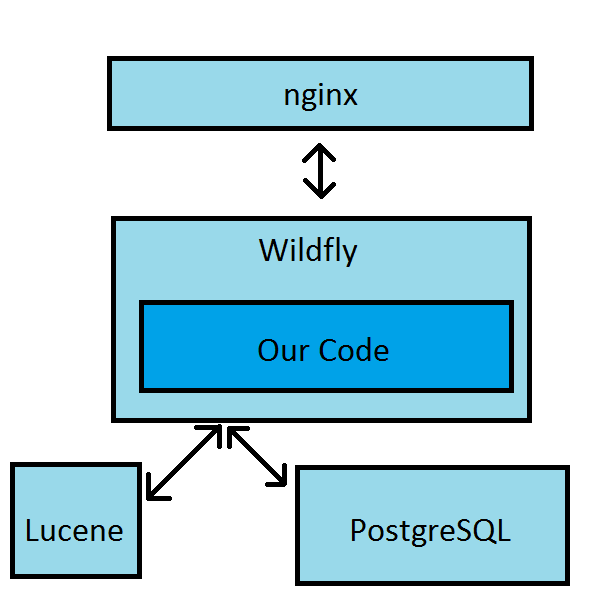
\includegraphics[width=0.6\textwidth]{dankarkitektur.png}
            \end{figure}
        \end{frame}

    \subsection{Data}
        \begin{frame}[t]{Developing the Back--End}\framesubtitle{The Model}
            \begin{figure}[htb]
                    \centering
                    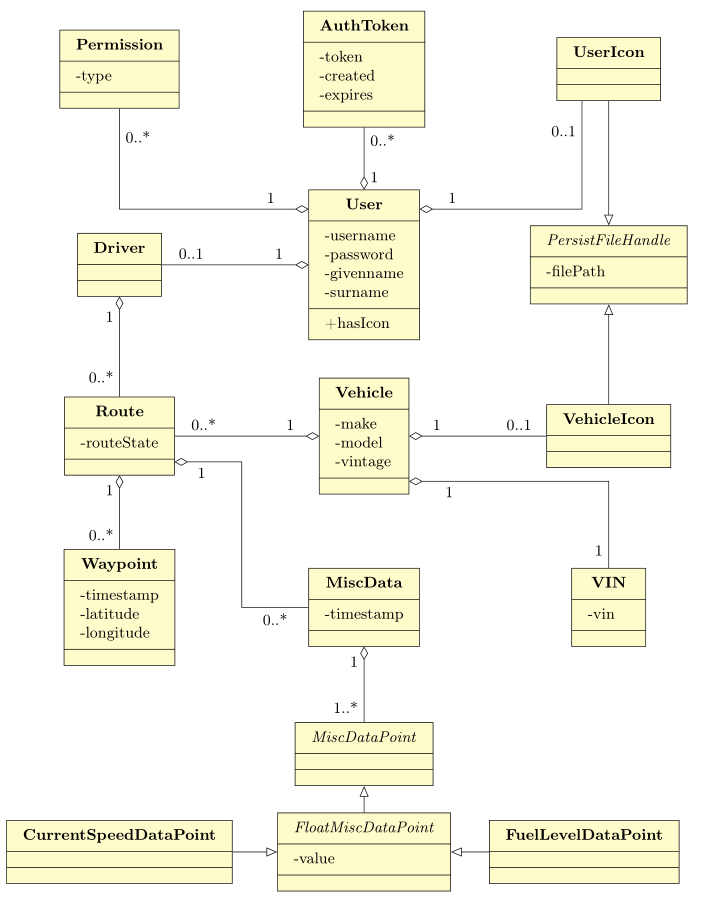
\includegraphics[width=0.55\textwidth]{class_diagram.png}
                \end{figure}
        \end{frame}

    \subsection{Endpoints}
        \begin{frame}[t]{Developing the Back--End}\framesubtitle{Services}
            The API is split into Services:
            \begin{itemize}
                \item AuthService
                \item UserService
                \item VehicleService
                \item RouteService
                \item WaypointService
                \item MiscDataService
            \end{itemize}
            Each has a distinct purpose
        \end{frame}
        \begin{frame}[t]{Developing the Back--End}\framesubtitle{API Endpoints}
\begin{table}[ht]
    \centering
    \scriptsize
    \begin{tabu} to \textwidth {llXl}
        HTTP Methods       & Endpoint               & Service     \\ \midrule
        \texttt{GET}, \texttt{POST} & /auth                    & \texttt{AuthService}\\ \tblgrpsep
        \texttt{GET}, \texttt{POST} & /user                    & \multirow{3}{*}{\texttt{UserService}}\\
        \texttt{GET}, \texttt{PUT}  & /user/\{uid\}            & \\
        \texttt{GET}, \texttt{PUT}  & /user/\{uid\}/icon       & \\ \tblgrpsep
        \texttt{GET}, \texttt{POST} & /vehicle                 & \multirow{3}{*}{\texttt{VehicleService}}\\
        \texttt{GET}, \texttt{PUT}  & /vehicle/\{vid\}         & \\
        \texttt{GET}, \texttt{PUT}  & /vehicle/\{vid\}/icon    & \\ \tblgrpsep
        \texttt{GET}, \texttt{POST} & /route                   & \multirow{2}{*}{\texttt{RouteService}}\\
        \texttt{GET}, \texttt{PUT}  & /route/\{rid\}           & \\
        \texttt{GET}, \texttt{POST} & /route/\{rid\}/waypoint  & \texttt{WaypointService}\\
        \texttt{GET}, \texttt{POST} & /route/\{rid\}/datapoint & \texttt{MiscDataService}\\
    \end{tabu}
    \caption{A table corrolating the endpoints and services.}\label{table:endpointservice}
\end{table}

        \end{frame}
    \subsection{Testing}
        \begin{frame}[t]{Developing the Back--End}\framesubtitle{Testing the Back--End Internally}
            \begin{itemize}
                \item Unit and Integration Tests
                \begin{itemize}
                    \item JUnit Testing Framework
                    \item Goal: Test all non--trivial code
                    \item Avoid Regressions when programming
                    \item 100 tests for the services
                    \item 54 tests for the persistence
                    \item Testing with a Database can lead to issues
                \end{itemize}
            \end{itemize}
\end{frame}
